% Options for packages loaded elsewhere
\PassOptionsToPackage{unicode}{hyperref}
\PassOptionsToPackage{hyphens}{url}
%
\documentclass[
]{article}
\usepackage{amsmath,amssymb}
\usepackage{iftex}
\ifPDFTeX
  \usepackage[T1]{fontenc}
  \usepackage[utf8]{inputenc}
  \usepackage{textcomp} % provide euro and other symbols
\else % if luatex or xetex
  \usepackage{unicode-math} % this also loads fontspec
  \defaultfontfeatures{Scale=MatchLowercase}
  \defaultfontfeatures[\rmfamily]{Ligatures=TeX,Scale=1}
\fi
\usepackage{lmodern}
\ifPDFTeX\else
  % xetex/luatex font selection
\fi
% Use upquote if available, for straight quotes in verbatim environments
\IfFileExists{upquote.sty}{\usepackage{upquote}}{}
\IfFileExists{microtype.sty}{% use microtype if available
  \usepackage[]{microtype}
  \UseMicrotypeSet[protrusion]{basicmath} % disable protrusion for tt fonts
}{}
\makeatletter
\@ifundefined{KOMAClassName}{% if non-KOMA class
  \IfFileExists{parskip.sty}{%
    \usepackage{parskip}
  }{% else
    \setlength{\parindent}{0pt}
    \setlength{\parskip}{6pt plus 2pt minus 1pt}}
}{% if KOMA class
  \KOMAoptions{parskip=half}}
\makeatother
\usepackage{xcolor}
\usepackage[margin=1in]{geometry}
\usepackage{color}
\usepackage{fancyvrb}
\newcommand{\VerbBar}{|}
\newcommand{\VERB}{\Verb[commandchars=\\\{\}]}
\DefineVerbatimEnvironment{Highlighting}{Verbatim}{commandchars=\\\{\}}
% Add ',fontsize=\small' for more characters per line
\usepackage{framed}
\definecolor{shadecolor}{RGB}{248,248,248}
\newenvironment{Shaded}{\begin{snugshade}}{\end{snugshade}}
\newcommand{\AlertTok}[1]{\textcolor[rgb]{0.94,0.16,0.16}{#1}}
\newcommand{\AnnotationTok}[1]{\textcolor[rgb]{0.56,0.35,0.01}{\textbf{\textit{#1}}}}
\newcommand{\AttributeTok}[1]{\textcolor[rgb]{0.13,0.29,0.53}{#1}}
\newcommand{\BaseNTok}[1]{\textcolor[rgb]{0.00,0.00,0.81}{#1}}
\newcommand{\BuiltInTok}[1]{#1}
\newcommand{\CharTok}[1]{\textcolor[rgb]{0.31,0.60,0.02}{#1}}
\newcommand{\CommentTok}[1]{\textcolor[rgb]{0.56,0.35,0.01}{\textit{#1}}}
\newcommand{\CommentVarTok}[1]{\textcolor[rgb]{0.56,0.35,0.01}{\textbf{\textit{#1}}}}
\newcommand{\ConstantTok}[1]{\textcolor[rgb]{0.56,0.35,0.01}{#1}}
\newcommand{\ControlFlowTok}[1]{\textcolor[rgb]{0.13,0.29,0.53}{\textbf{#1}}}
\newcommand{\DataTypeTok}[1]{\textcolor[rgb]{0.13,0.29,0.53}{#1}}
\newcommand{\DecValTok}[1]{\textcolor[rgb]{0.00,0.00,0.81}{#1}}
\newcommand{\DocumentationTok}[1]{\textcolor[rgb]{0.56,0.35,0.01}{\textbf{\textit{#1}}}}
\newcommand{\ErrorTok}[1]{\textcolor[rgb]{0.64,0.00,0.00}{\textbf{#1}}}
\newcommand{\ExtensionTok}[1]{#1}
\newcommand{\FloatTok}[1]{\textcolor[rgb]{0.00,0.00,0.81}{#1}}
\newcommand{\FunctionTok}[1]{\textcolor[rgb]{0.13,0.29,0.53}{\textbf{#1}}}
\newcommand{\ImportTok}[1]{#1}
\newcommand{\InformationTok}[1]{\textcolor[rgb]{0.56,0.35,0.01}{\textbf{\textit{#1}}}}
\newcommand{\KeywordTok}[1]{\textcolor[rgb]{0.13,0.29,0.53}{\textbf{#1}}}
\newcommand{\NormalTok}[1]{#1}
\newcommand{\OperatorTok}[1]{\textcolor[rgb]{0.81,0.36,0.00}{\textbf{#1}}}
\newcommand{\OtherTok}[1]{\textcolor[rgb]{0.56,0.35,0.01}{#1}}
\newcommand{\PreprocessorTok}[1]{\textcolor[rgb]{0.56,0.35,0.01}{\textit{#1}}}
\newcommand{\RegionMarkerTok}[1]{#1}
\newcommand{\SpecialCharTok}[1]{\textcolor[rgb]{0.81,0.36,0.00}{\textbf{#1}}}
\newcommand{\SpecialStringTok}[1]{\textcolor[rgb]{0.31,0.60,0.02}{#1}}
\newcommand{\StringTok}[1]{\textcolor[rgb]{0.31,0.60,0.02}{#1}}
\newcommand{\VariableTok}[1]{\textcolor[rgb]{0.00,0.00,0.00}{#1}}
\newcommand{\VerbatimStringTok}[1]{\textcolor[rgb]{0.31,0.60,0.02}{#1}}
\newcommand{\WarningTok}[1]{\textcolor[rgb]{0.56,0.35,0.01}{\textbf{\textit{#1}}}}
\usepackage{longtable,booktabs,array}
\usepackage{calc} % for calculating minipage widths
% Correct order of tables after \paragraph or \subparagraph
\usepackage{etoolbox}
\makeatletter
\patchcmd\longtable{\par}{\if@noskipsec\mbox{}\fi\par}{}{}
\makeatother
% Allow footnotes in longtable head/foot
\IfFileExists{footnotehyper.sty}{\usepackage{footnotehyper}}{\usepackage{footnote}}
\makesavenoteenv{longtable}
\usepackage{graphicx}
\makeatletter
\def\maxwidth{\ifdim\Gin@nat@width>\linewidth\linewidth\else\Gin@nat@width\fi}
\def\maxheight{\ifdim\Gin@nat@height>\textheight\textheight\else\Gin@nat@height\fi}
\makeatother
% Scale images if necessary, so that they will not overflow the page
% margins by default, and it is still possible to overwrite the defaults
% using explicit options in \includegraphics[width, height, ...]{}
\setkeys{Gin}{width=\maxwidth,height=\maxheight,keepaspectratio}
% Set default figure placement to htbp
\makeatletter
\def\fps@figure{htbp}
\makeatother
\setlength{\emergencystretch}{3em} % prevent overfull lines
\providecommand{\tightlist}{%
  \setlength{\itemsep}{0pt}\setlength{\parskip}{0pt}}
\setcounter{secnumdepth}{-\maxdimen} % remove section numbering
\usepackage{amsmath}
\usepackage{mathtools}
\usepackage{amsthm}
\usepackage{hhline}
\ifLuaTeX
  \usepackage{selnolig}  % disable illegal ligatures
\fi
\IfFileExists{bookmark.sty}{\usepackage{bookmark}}{\usepackage{hyperref}}
\IfFileExists{xurl.sty}{\usepackage{xurl}}{} % add URL line breaks if available
\urlstyle{same}
\hypersetup{
  pdftitle={Time Series Analysis - 478 - HW \#3},
  pdfauthor={Alex Towell (atowell@siue.edu)},
  hidelinks,
  pdfcreator={LaTeX via pandoc}}

\title{Time Series Analysis - 478 - HW \#3}
\author{Alex Towell
(\href{mailto:atowell@siue.edu}{\nolinkurl{atowell@siue.edu}})}
\date{}

\begin{document}
\maketitle

\newcommand{\var}{\operatorname{Var}}
\newcommand{\expect}{\operatorname{E}}
\newcommand{\corr}{\operatorname{Corr}}
\newcommand{\cov}{\operatorname{Cov}}
\newcommand{\ssr}{\operatorname{SSR}}
\newcommand{\se}{\operatorname{SE}}
\newcommand{\mat}[1]{\mathbf{#1}} 
\newcommand{\eval}[2]{\left. #1 \right\vert_{#2}}

\hypertarget{problem-1}{%
\section{Problem 1}\label{problem-1}}

Regression through the origin: We will consider a special case of simple
linear regression where the intercept is assumed to be zero from the
outset. Let \[
   Y i = \beta x_i + \epsilon_i\,,
\] where \(\operatorname{E}(\epsilon_i) = 0\) and
\(\operatorname{Var}(\epsilon_i) = \sigma^2\).

\hypertarget{part-a}{%
\subsection{Part (A)}\label{part-a}}

\fbox{
Define $Q(\beta) \coloneqq \sum_{i=1}^{n} (Y_i - \beta x_i)^2$.
the minimizer of $Q(\beta)$ is $\hat\beta = \frac{\sum x_i Y_i}{\sum x_i^2}$.}

\begin{proof}
The function to minimize is given by
\begin{equation}
   Q(\beta) = \sum_{i=1}^{n} (Y_i - \beta x_i)^2\,,
\end{equation}
which has a minimum when its derivative is zero,
\begin{align*}
   \left. \frac{\mathrm{d}Q}{\mathrm{d}\beta} \right\vert_{\hat\beta} = 0\\
   -2 \sum (Y_i - \hat\beta x_i) x_i = 0\\
   \sum Y_i x_i = \hat\beta \sum x_i^2\,.
\end{align*}
Solving for $\hat\beta$,
\begin{equation}
   \hat\beta = \frac{ \sum Y_i x_i }{\sum x_i^2}\,.
\end{equation}
\end{proof}

\hypertarget{part-b}{%
\subsection{Part (B)}\label{part-b}}

\fbox{
Show $\operatorname{E}(\hat\beta) = \beta$.}
\begin{proof}
The expectation of $\hat\beta$ is given by
\begin{align*}
   \operatorname{E}(\hat\beta) &= \operatorname{E}\left(\frac{ \sum Y_i x_i }{\sum x_i^2}\right)\\
                      %&= \frac{\expect(\sum Y_i x_i)}{\sum x_i^2}\\
                      &= \frac{\sum \operatorname{E}(Y_i x_i)}{\sum x_i^2}\\
                      %&= \frac{\sum x_i \expect(Y_i)}{\sum x_i^2}\\
                      &= \frac{\sum x_i \operatorname{E}(\beta x_i + \epsilon_i)}{\sum x_i^2}\\
                      &= \frac{\beta \sum x^2_i}{\sum x_i^2}\,,
\end{align*}
which finally can be simplified to
\begin{equation}
   \operatorname{E}(\hat\beta) = \beta\,.
\end{equation}
\end{proof}

\hypertarget{part-c}{%
\subsection{Part (C)}\label{part-c}}

\fbox{
Show $\operatorname{Var}(\hat\beta) = \frac{\sigma^2}{\sum x^2_i}$.}

\begin{proof}
The variance of $\hat\beta$ is given by
\begin{align*}
   \operatorname{Var}(\hat\beta) &= \left(\sum x_i^2\right)^{-2}\operatorname{Var}\left(\sum Y_i x_i\right)\\
                   %&= \left(\sum x_i^2\right)^{-2}\sum \var(Y_i x_i)\\
                   &= \left(\sum x_i^2\right)^{-2}\sum x_i^2 \operatorname{Var}(Y_i)\\
                   &= \left(\sum x_i^2\right)^{-2}\sum x_i^2 \operatorname{Var}(\beta x_i + \epsilon_i)\\
                   &= \left(\sum x_i^2\right)^{-2}\sum x_i^2 \operatorname{Var}(\epsilon_i)\\
                   &= \sigma^2 \left(\sum x_i^2\right)^{-2} \sum x_i^2
\end{align*}
which finally can be simplified to
\begin{equation}
   \operatorname{Var}(\hat\beta) = \sigma^2 \left(\sum x_i^2\right)^{-1}\,.
\end{equation}
\end{proof}

\hypertarget{part-d}{%
\subsection{Part (D)}\label{part-d}}

\fbox{
Write the model as $\mathbf{Y} = \mathbf{X} \beta + \mathbf{\epsilon}$.}

The equation
\(\mathbf{Y} = \mathbf{X} \mathbf{\beta }+ \mathbf{\epsilon}\) can be
rewritten as \begin{equation}
   \begin{pmatrix}
       Y_1\\
       Y_2\\
       \vdots\\
       Y_n
   \end{pmatrix}
   =
   \begin{pmatrix}
       x_1\\
       x_2\\
       \vdots\\
       x_n
   \end{pmatrix}
   \beta
   +
   \begin{pmatrix}
       \epsilon_1\\
       \epsilon_2\\
       \vdots\\
       \epsilon_n
   \end{pmatrix}\,.
\end{equation}

\begin{proof}
The original model is given by
$$
   Y_i \coloneqq \beta x_i + \epsilon_i\,.
$$

When we perform the calculation $\mathbf{Y} = \mathbf{X} \beta$, the $i$-th element of
$\mathbf{Y}$ is $Y_i = \beta x_i + \epsilon_i$.
\end{proof}

\hypertarget{part-e}{%
\subsection{Part (E)}\label{part-e}}

\fbox{Verify $\hat\beta = (\mathbf{X}' \mathbf{X})^{-1}\mathbf{X}' \mathbf{Y}$ is equivalent to the minimizer in Part (A).}

\begin{proof}
To show that $\hat\beta = (\mathbf{X}'\mathbf{X})^{-1} \mathbf{X}'\mathbf{Y} = \frac{\sum x_i Y_i}{\sum x_i^2}$,
we apply the matrix operations to demonstrate equivalence to Part (A).

The transpose of $\mathbf{X}$ is $\mathbf{X}' = (x_1 \, x_2 \, \cdots \, x_n)$, a row vector. Making the
appropriate substitutions, we get
\begin{equation}
\hat\beta = \left(
   (x_1 \, x_2 \, \cdots \, x_n)
   \begin{pmatrix}
       x_1\\
       x_2\\
       \vdots\\
       x_n
   \end{pmatrix}
   \right)^{-1}
   (x_1 \, x_2 \, \cdots \, x_n)
   \begin{pmatrix}
       Y_1\\
       Y_2\\
       \vdots\\
       Y_n
   \end{pmatrix}\,.
\end{equation}

We see that $X'X$ is just the sum of squares $x_1^2 + \cdots + x_n^2$ and
$X'Y$ is just $x_1 Y_1 + \cdots + x_n Y_n$, resulting in
\begin{equation*}
\hat\beta = (x^2_1 + x^2_2 + \cdots + x^2_n)^{-1}
   (x_1 Y_1 + x_2 Y_2 + \cdots + x_n Y_n)\,.
\end{equation*}
Since the inverse operation $^{-1} \colon \mathbb{R} \mapsto \mathbb{R}$ is just the reciprocal,
we may rewrite the above as
\begin{equation*}
   \hat\beta = \frac{x_1 Y_1 + x_2 Y_2 + \cdots + x_n Y_n}{x^2_1 + x^2_2 + \cdots + x^2_n}\,.
\end{equation*}
which may finally rewritten as
\begin{equation}
\hat\beta = \frac{\sum x_i Y_i}{\sum x_i^2}\,.
\end{equation}
\end{proof}

\hypertarget{part-f}{%
\subsection{Part (F)}\label{part-f}}

\fbox{Show that $\operatorname{Var}(\hat\beta) = \sigma^2(\mathbf{X}' \mathbf{X})^{-1}$ is equivalent to the scalar form in Part (C).}

\begin{proof}
The variance of $\hat\beta$ is given by
\begin{equation}
   \operatorname{Var}(\hat\beta) = \operatorname{Var}\left((\mathbf{X}'\mathbf{X})^{-1} \mathbf{X}' \mathbf{Y}\right)\,.
\end{equation}
Note that the variance of a random vector $\mathbf{T}$ multiplied on the left
by a vector $\mathbf{U}$ is given by
\begin{equation}
   \operatorname{Var}(\mathbf{U} \mathbf{T}) = \mathbf{U} \operatorname{Var}(\mathbf{T}) \mathbf{U'}\,.
\end{equation}
Thus,
\begin{equation}
   \operatorname{Var}(\hat\beta) = \left((\mathbf{X}'\mathbf{X})^{-1} \mathbf{X}'\right)\operatorname{Var}(\mathbf{Y})\left((\mathbf{X}'\mathbf{X})^{-1} \mathbf{X}'\right)'\,.
\end{equation}
By the property of transposition, $(\mathbf{A}\mathbf{B})' = \mathbf{B}'\mathbf{A}'$, we may rewrite the above as
$$
   \operatorname{Var}(\hat\beta) = (\mathbf{X}'\mathbf{X})^{-1} \mathbf{X}' \operatorname{Var}(\mathbf{Y}) \mathbf{X} (\mathbf{X}'\mathbf{X})^{-T}\,.
$$
By the assumption that $\{\epsilon_i\}$ are i.i.d., the variance of $\mathbf{Y}$
is $\sigma^2 \mathbf{I}_{p}$,
\begin{align*}   
   \operatorname{Var}(\hat\beta) &= (\mathbf{X}'\mathbf{X})^{-1} \mathbf{X}'
   \sigma^2 \mathbf{I}
   \mathbf{X} (\mathbf{X}'\mathbf{X})^{-T}\\
   &= \sigma^2 (\mathbf{X}'\mathbf{X})^{-1} \mathbf{X}'
   \mathbf{X} (\mathbf{X}'\mathbf{X})^{-T}\\
   &= \sigma^2  (\mathbf{X}'\mathbf{X})^{-T}\,.
\end{align*}
Given a symmetric matrix $\mathbf{A}$, $\mathbf{A}' = \mathbf{A}$.
Since $\mathbf{X}' \mathbf{X}$ is ``symmetric'' (a scalar value, being viewed as
a matrix, is by definition symmetric), we can simplify the above to
\begin{align*}
   \operatorname{Var}(\hat\beta) = \sigma^2  (\mathbf{X}'\mathbf{X})^{-1}\,.
\end{align*}
\end{proof}

Observe that since \(\hat\beta = c \mathbf{Y}\) where \(c\) is constant
and \(\mathbf{Y}\) is a vector of normals, \(\hat\beta\) is normally
distributed
\(\hat\beta \sim \mathcal{N}(\beta, \operatorname{Var}(\hat\beta))\).

\hypertarget{problem-2}{%
\section{Problem 2}\label{problem-2}}

Burple, Stephens, and Gloopshire (2014) report on a study in the Journal
of Questionable Research. Data were collected on the number of minutes
\(Y_i\) it took \(n = 237\) Glippers to learn how to drive a small,
motorized car. Two predictors of interest are the estimated age of the
glipper in months \(x_{i 1}\) and the Glippers Maladaptive Score (GMS)
\(x_{i 2}\), a number from \(50\) to \(100\) that summarizes how poor
the glipper's vision is. Consider the following multiple regression
output from R.

\begin{longtable}[]{@{}lrl@{}}
\caption{Regression output from R}\tabularnewline
\toprule\noalign{}
Coefficients & Estimate & Std. Error \\
\midrule\noalign{}
\endfirsthead
\toprule\noalign{}
Coefficients & Estimate & Std. Error \\
\midrule\noalign{}
\endhead
\bottomrule\noalign{}
\endlastfoot
(Intercept) & -182.57923 & 7.41169 \\
Age & 8.56069 & 0.31150 \\
GMS & 0.28066 & 0.04621 \\
\end{longtable}

\begin{longtable}[]{@{}llll@{}}
\caption{Anaylysis of Variance Table}\tabularnewline
\toprule\noalign{}
type & df & ss & ms \\
\midrule\noalign{}
\endfirsthead
\toprule\noalign{}
type & df & ss & ms \\
\midrule\noalign{}
\endhead
\bottomrule\noalign{}
\endlastfoot
regression & & & \\
error & & 23565 & \\
total & 236 & 104682 & \\
\end{longtable}

\hypertarget{common-code}{%
\subsection{Common code}\label{common-code}}

The following R code is used to produce many of the answers to this
problem set.

\begin{Shaded}
\begin{Highlighting}[]
\NormalTok{n }\OtherTok{\textless{}{-}} \DecValTok{237}
\NormalTok{p }\OtherTok{\textless{}{-}} \DecValTok{3}
\NormalTok{ss.e }\OtherTok{\textless{}{-}} \DecValTok{23565}
\NormalTok{ss.t }\OtherTok{\textless{}{-}} \DecValTok{104682}

\CommentTok{\# ss.e + ss.r = ss.t =\textgreater{} ss.r = ss.t {-} ss.e}
\NormalTok{ss.r }\OtherTok{\textless{}{-}}\NormalTok{ ss.t }\SpecialCharTok{{-}}\NormalTok{ ss.e}

\NormalTok{df.r }\OtherTok{\textless{}{-}}\NormalTok{ p}\DecValTok{{-}1}
\NormalTok{df.e }\OtherTok{\textless{}{-}}\NormalTok{ n}\SpecialCharTok{{-}}\NormalTok{p}
\NormalTok{df.t }\OtherTok{\textless{}{-}}\NormalTok{ n}\DecValTok{{-}1}

\NormalTok{ms.r }\OtherTok{\textless{}{-}}\NormalTok{ ss.r }\SpecialCharTok{/}\NormalTok{ df.r}
\NormalTok{ms.e }\OtherTok{\textless{}{-}}\NormalTok{ ss.e }\SpecialCharTok{/}\NormalTok{ df.e}

\CommentTok{\# sample variance}
\NormalTok{ms.t }\OtherTok{\textless{}{-}}\NormalTok{ ss.t }\SpecialCharTok{/}\NormalTok{ df.t}

\NormalTok{B0.est }\OtherTok{\textless{}{-}} \SpecialCharTok{{-}}\FloatTok{182.57923}
\NormalTok{B1.est }\OtherTok{\textless{}{-}} \FloatTok{8.56069}
\NormalTok{B2.est }\OtherTok{\textless{}{-}} \FloatTok{0.28066}

\NormalTok{B0.se }\OtherTok{\textless{}{-}} \FloatTok{7.41169}
\NormalTok{B1.se }\OtherTok{\textless{}{-}} \FloatTok{0.31150}
\NormalTok{B2.se }\OtherTok{\textless{}{-}} \FloatTok{0.04621}
\end{Highlighting}
\end{Shaded}

\hypertarget{part-a-1}{%
\subsection{Part (A)}\label{part-a-1}}

\fbox{Complete the ANOVA table.}

There are \(p = 3\) parameters in the model and it is given that there
are \(n = 237\) observations with a sum of squared error
\(\rm{SS_E} = 23565\) and sum of squared total \(\rm{SS_T} = 104682\).

From this given information, we may compute the remaining values in the
ANOVA table by observing the following set of relationships:
\begin{align*}
   \rm{SS_R} &= \rm{SS_T} - \rm{SS_E}\\
   \rm{MS_R} &= \rm{SS_R} / \rm{df_R}\\
   \rm{MS_E} &= \rm{SS_E} / \rm{df_E}\\
   \rm{MS_T} &= \rm{SS_T} / \rm{df_T}
\end{align*} where \(\rm{df}_R = p-1\), \(\rm{df}_E = n-p\), and
\(\rm{df}_T = n-1\).

We output the ANOVA table with the following R code:

\begin{Shaded}
\begin{Highlighting}[]
\NormalTok{anova\_table }\OtherTok{\textless{}{-}} \FunctionTok{data.frame}\NormalTok{(}
   \AttributeTok{type =} \FunctionTok{c}\NormalTok{(}\StringTok{"regression"}\NormalTok{,}\StringTok{"residual"}\NormalTok{,}\StringTok{"total"}\NormalTok{), }
   \AttributeTok{ss =} \FunctionTok{c}\NormalTok{(ss.r,ss.e,ss.t),}
   \AttributeTok{dof =} \FunctionTok{c}\NormalTok{(df.r,df.e,df.t),}
   \AttributeTok{ms =} \FunctionTok{c}\NormalTok{(ms.r,ms.e,ms.t)}
\NormalTok{)}
\NormalTok{knitr}\SpecialCharTok{::}\FunctionTok{kable}\NormalTok{(anova\_table, }\AttributeTok{digits=}\DecValTok{2}\NormalTok{, }\AttributeTok{caption =} \StringTok{"ANOVA table."}\NormalTok{)}
\end{Highlighting}
\end{Shaded}

\begin{longtable}[]{@{}lrrr@{}}
\caption{ANOVA table.}\tabularnewline
\toprule\noalign{}
type & ss & dof & ms \\
\midrule\noalign{}
\endfirsthead
\toprule\noalign{}
type & ss & dof & ms \\
\midrule\noalign{}
\endhead
\bottomrule\noalign{}
\endlastfoot
regression & 81117 & 2 & 40558.50 \\
residual & 23565 & 234 & 100.71 \\
total & 104682 & 236 & 443.57 \\
\end{longtable}

\hypertarget{part-b-1}{%
\subsection{Part (B)}\label{part-b-1}}

\fbox{%
\begin{minipage}{.8\textwidth}
Calculate the F-statistic from the ANOVA table and use it to test
$$
H_0 \colon \beta_1 = \beta_2 = 0\,.
$$
What does this imply about $\beta_1$ and $\beta_2$?
\end{minipage}}

Consider the model \begin{equation}
  Y_i = \beta_0 + \beta_1 x_1 + \beta_2 x_2 + \epsilon_i
\end{equation} where \(x_1\) and \(x_2\) are the independent predictor
variables.

If we wish to do an overall test on the model, then we are interested in
the hypothesis test \begin{align*}
   H_0 &\colon \beta_1 = \beta_2 = 0\,\\
   H_1 &\colon \beta_1 \neq 0 \lor \beta_2 \neq 0\,.
\end{align*}

Rejection of \(H_0\) implies that one or more predictors is signficant
in the model.

If \(H_0\) is true and the model errors are normal and independent with
constant variance, then the test statistic for significance of
regression is \begin{equation}
    F_0 = \frac{\rm{SS_R} / (p-1)}{\rm{SS_E}/(n-p)} = \frac{\rm{MS_R}}{\rm{MS_E}}\,,
\end{equation} where \(F_0 \sim F(p-1,n-p)\).

We compute the statistic using the following R code:

\begin{Shaded}
\begin{Highlighting}[]
\NormalTok{F.ratio}\OtherTok{=}\NormalTok{ms.r}\SpecialCharTok{/}\NormalTok{ms.e}
\NormalTok{p\_value}\OtherTok{=}\DecValTok{1}\SpecialCharTok{{-}}\FunctionTok{pf}\NormalTok{(F.ratio,p,n}\SpecialCharTok{{-}}\NormalTok{p) }\CommentTok{\#p{-}value from the F test}
\FunctionTok{cat}\NormalTok{(}\StringTok{"test statistic F0 ="}\NormalTok{,F.ratio, }\StringTok{"with p{-}value"}\NormalTok{, p\_value, }\StringTok{"}\SpecialCharTok{\textbackslash{}n}\StringTok{"}\NormalTok{)}
\end{Highlighting}
\end{Shaded}

\begin{verbatim}
## test statistic F0 = 402.7451 with p-value 0
\end{verbatim}

We see that \(\Pr(F_0 > 3) \approx 0.05\). We have a much larger value
and we see that the \(p\)-value is essentially \(0\). Thus, we have very
strong evidence to reject the null hypothesis, i.e., either \(\beta_1\)
or \(\beta_2\) (or both) are not zero and we conclude that one or more
of the predictors in the model is significant.

\hypertarget{part-c-1}{%
\subsection{Part (C)}\label{part-c-1}}

\fbox{
\begin{minipage}{.8\textwidth}
Report each of $\hat\beta_1$ and $\hat\beta_2$.
Construct $t$-tests $H_0 \colon \beta_1 = 0$ and $H_0 \colon \beta_2 = 0$
individually.
Can either predictor be dropped in the presence of the other?
\end{minipage}
}

Observe
\(\hat\beta \sim \mathcal{N}(\mathbf{\beta}, \sigma^2 \mathbf{C})\) and
therefore \(\hat\beta_j \sim \mathcal(\beta_j, \sigma^2 C_{j j})\).
Thus,
\(\frac{\hat\beta_j - \beta_j}{\sqrt(\sigma^2 C_{j j})} \sim \mathcal{N}(0,1)\).
Since we do not know \(\sigma^2\), we estimate it with
\(\hat\sigma^2 = \rm{MS_E}\), in which case

\[
   \frac{\hat\beta_j - \beta_j}{\operatorname{SE}(\hat\beta_j)} \sim t(\rm{df} = n-p)\,,
\] where
\(\operatorname{SE}(\hat\beta_j) \coloneqq \sqrt{\hat\sigma^2 C_{j j}}\)
is denoted the standard error and
\(\mathbf{C} \coloneqq (\mathbf{X}' \mathbf{X})^{-1}\).

We consider the hypothesis test for testing the significance of
\(\beta_j\), \begin{align*}
  H_0 : \beta_j = 0\,,\\
  H_1 : \beta_j \neq 0\,,
\end{align*} with test statistic \[
    t_0 = \frac{\hat\beta_j}{\operatorname{SE}(\hat\beta_j)} \sim t(\rm{df}=n-p)\,.
\] We reject \(H_0\) if \(t_0\) has a sufficiently small \(p\)-value,
where \[
   \text{$p$-value} = 2 \Pr(t < -|t_0|)\,.
\] We specify that we reject \(H_0\) if
\(p\text{-value} \leq \alpha = 0.05\) (or equivalently
\(|t_0| > t_{\alpha/2,n-p}\)).

\begin{Shaded}
\begin{Highlighting}[]
\NormalTok{B1.t0 }\OtherTok{\textless{}{-}}\NormalTok{ B1.est }\SpecialCharTok{/}\NormalTok{ B1.se}
\NormalTok{B2.t0 }\OtherTok{\textless{}{-}}\NormalTok{ B2.est }\SpecialCharTok{/}\NormalTok{ B2.se}
\FunctionTok{cat}\NormalTok{(}\StringTok{"B1.t0 ="}\NormalTok{,B1.t0,}\StringTok{"}\SpecialCharTok{\textbackslash{}n}\StringTok{"}\NormalTok{)}
\end{Highlighting}
\end{Shaded}

\begin{verbatim}
## B1.t0 = 27.48215
\end{verbatim}

\begin{Shaded}
\begin{Highlighting}[]
\FunctionTok{cat}\NormalTok{(}\StringTok{"B2.t0 ="}\NormalTok{,B2.t0,}\StringTok{"}\SpecialCharTok{\textbackslash{}n}\StringTok{"}\NormalTok{)}
\end{Highlighting}
\end{Shaded}

\begin{verbatim}
## B2.t0 = 6.073577
\end{verbatim}

\begin{Shaded}
\begin{Highlighting}[]
\CommentTok{\#p{-}value from the T test}
\NormalTok{B1.pval}\OtherTok{=}\DecValTok{2}\SpecialCharTok{*}\FunctionTok{pt}\NormalTok{(}\SpecialCharTok{{-}}\DecValTok{1}\SpecialCharTok{*}\FunctionTok{abs}\NormalTok{(B1.t0),}\AttributeTok{df=}\NormalTok{n}\SpecialCharTok{{-}}\NormalTok{p)}
\NormalTok{B2.pval}\OtherTok{=}\DecValTok{2}\SpecialCharTok{*}\FunctionTok{pt}\NormalTok{(}\SpecialCharTok{{-}}\DecValTok{1}\SpecialCharTok{*}\FunctionTok{abs}\NormalTok{(B2.t0),}\AttributeTok{df=}\NormalTok{n}\SpecialCharTok{{-}}\NormalTok{p)}
\FunctionTok{cat}\NormalTok{(}\StringTok{"B1 pvalue ="}\NormalTok{,B1.pval,}\StringTok{",B2 pvalue ="}\NormalTok{, B2.pval)}
\end{Highlighting}
\end{Shaded}

\begin{verbatim}
## B1 pvalue = 3.321975e-75 ,B2 pvalue = 5.019091e-09
\end{verbatim}

It is given that \(\hat\beta_1 = 8.56\) and \(\hat\beta_2 = 0.28\)
respectively with standard errors \(0.31150\) and \(0.04621\) and
\(p\)-values of \(3.321975e^{-75}\) and \(5.019091e^{-09}\). These
\(p\)-values are practically \emph{zero} and thus in the presence in the
presence of the other, neither predictor should be dropped.

\hypertarget{part-d-1}{%
\subsection{Part (D)}\label{part-d-1}}

\fbox{Interpret both coefficients.}

The estimated coefficients in the model are given by
\(\hat\beta_1 = 8.56\) and \(\hat\beta_2 = 0.28\), thus

\begin{equation}
\hat{Y}_i = \hat\beta_0 + 8.56 x_{i 1} + 0.28 x_{i 2} + \epsilon_i
\end{equation} which has an estimated expectation \begin{equation}
E(\hat{Y}_i) = \hat\beta_0 + 8.56 x_{i 1} + 0.28 x_{i 2}\,,
\end{equation} where \(x_{i 1}\) is the estimated age of the glipper in
months, \(x_{i 2}\) is the Glippers Maladaptive Score (GMS), a number
between \(50\) and \(100\) that summarizes how poor the glipper's vision
is, and \(\hat{Y}_i\) is the number of minutes it takes a glipper to
learn how to drive a small, motorized car with those predictors.

According to the model, the rate of increase with respect to age and GMA
is expected to increase the number of minutes to learn by \(8.56\) and
\(0.28\) minutes respectively.

\hypertarget{part-e-1}{%
\subsection{Part (E)}\label{part-e-1}}

\fbox{Report $R^2$; how is it interpretted here?}

Recall that \(R^2 = SS_R / SS_T = 1 - SS_E / SS_T\). Thus, it is the
percentage of the variability explained by the regression model versus
the total variability. All things else being equal, the more of the
variability we can explain by the regression model the better. Since
\(R^2\) is a number between \(0\) and \(1\), the closer to \(1\) the
better.

We run the following R code:

\begin{Shaded}
\begin{Highlighting}[]
\CommentTok{\#R2 \textless{}{-} 1 {-} ss.e / ss.t}
\NormalTok{R2 }\OtherTok{\textless{}{-}}\NormalTok{ ss.r }\SpecialCharTok{/}\NormalTok{ ss.t}
\FunctionTok{cat}\NormalTok{(}\StringTok{"R2 ="}\NormalTok{,R2,}\StringTok{"}\SpecialCharTok{\textbackslash{}n}\StringTok{"}\NormalTok{)}
\end{Highlighting}
\end{Shaded}

\begin{verbatim}
## R2 = 0.7748897
\end{verbatim}

We see that \(R^2 \approx 0.77\), and thus the model explains around
\(77\%\) of the variability in the data.

Note that a large value of \(R^2\) does not necessarily imply the model
is good, since we can always capture more variability in a model by
adding more parameters to it, which contributes to \emph{over-fitting}
the particulars of the observe data.

\hypertarget{problem-3}{%
\section{Problem 3}\label{problem-3}}

Consider the ''mtcars'' data in R. You can load and view the dataset by
typing ''mtcars'' in R console. Consider the response variable mileage
per hour (\(Y=\rm{mpg}\)), and two predictors, horsepower and weight
\((X_1 = \rm{hp}, X_2 = \rm{wt})\). Ignore other variables for now.

\hypertarget{part-a-2}{%
\subsection{Part (A)}\label{part-a-2}}

\fbox{
\begin{minipage}{.8\textwidth}
Obtain and report the scatterplot matrix; what does it tell you about the relationship between mpg and each of the predictors, horsepower and weight?
\end{minipage}}

We print out the scatterplot matrix with the following R code.

\begin{Shaded}
\begin{Highlighting}[]
\FunctionTok{pairs}\NormalTok{(mpg}\SpecialCharTok{\textasciitilde{}}\NormalTok{hp}\SpecialCharTok{+}\NormalTok{wt,mtcars, }\AttributeTok{main=}\StringTok{"Scatterplot Matrix"}\NormalTok{)      }\CommentTok{\#construct scatterplots }
\end{Highlighting}
\end{Shaded}

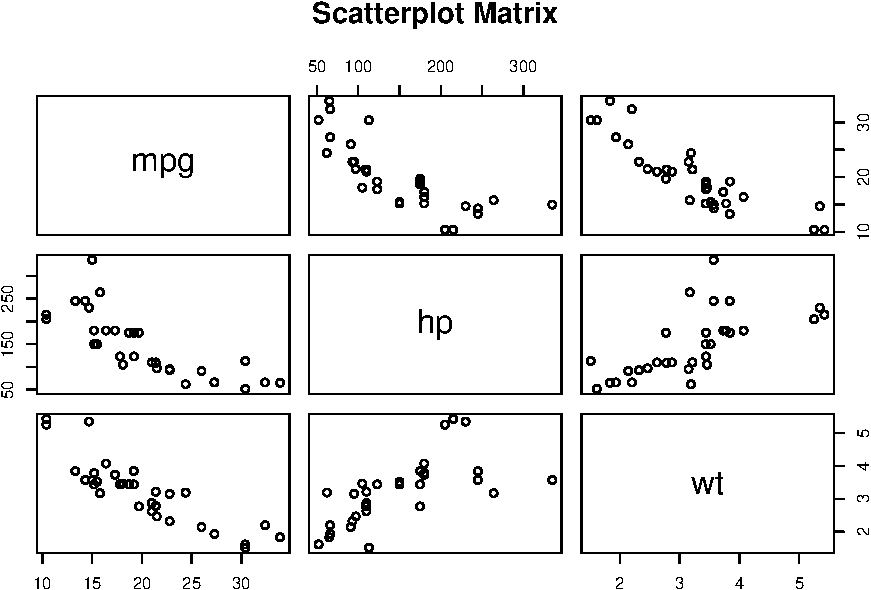
\includegraphics{hw3_files/figure-latex/unnamed-chunk-6-1.pdf}

The scatter plot visually indicates that the miles per gallon (mpg) is
negatively correlated with both the horsepower (hp) and the weight (wt).

\hypertarget{part-b-2}{%
\subsection{Part (B)}\label{part-b-2}}

\fbox{
\begin{minipage}{.8\textwidth}
Fit the regression model $Y_i = \beta_0 + \beta_1 x_{i 1} + \beta_2 x_{i 2} + \epsilon_i$.
Report the ANOVA table and the table of regression coefficients.
\end{minipage}
}

We use the following R code to fit the model and then report the ANOVA
table.

\begin{Shaded}
\begin{Highlighting}[]
\DocumentationTok{\#\#\#\# Regression Analysis Using lm() \#\#\#\#}

\CommentTok{\# fit a multiple regression model}
\NormalTok{mpg\_hp\_wt.model}\OtherTok{=}\FunctionTok{lm}\NormalTok{(mpg}\SpecialCharTok{\textasciitilde{}}\NormalTok{hp}\SpecialCharTok{+}\NormalTok{wt, }\AttributeTok{data=}\NormalTok{mtcars)}

\CommentTok{\# get details from the regression output}
\FunctionTok{summary}\NormalTok{(mpg\_hp\_wt.model)}
\end{Highlighting}
\end{Shaded}

\begin{verbatim}
## 
## Call:
## lm(formula = mpg ~ hp + wt, data = mtcars)
## 
## Residuals:
##    Min     1Q Median     3Q    Max 
## -3.941 -1.600 -0.182  1.050  5.854 
## 
## Coefficients:
##             Estimate Std. Error t value Pr(>|t|)    
## (Intercept) 37.22727    1.59879  23.285  < 2e-16 ***
## hp          -0.03177    0.00903  -3.519  0.00145 ** 
## wt          -3.87783    0.63273  -6.129 1.12e-06 ***
## ---
## Signif. codes:  0 '***' 0.001 '**' 0.01 '*' 0.05 '.' 0.1 ' ' 1
## 
## Residual standard error: 2.593 on 29 degrees of freedom
## Multiple R-squared:  0.8268, Adjusted R-squared:  0.8148 
## F-statistic: 69.21 on 2 and 29 DF,  p-value: 9.109e-12
\end{verbatim}

\begin{Shaded}
\begin{Highlighting}[]
\CommentTok{\# get the anova table}
\FunctionTok{anova}\NormalTok{(mpg\_hp\_wt.model)}
\end{Highlighting}
\end{Shaded}

\begin{verbatim}
## Analysis of Variance Table
## 
## Response: mpg
##           Df Sum Sq Mean Sq F value    Pr(>F)    
## hp         1 678.37  678.37 100.862 5.987e-11 ***
## wt         1 252.63  252.63  37.561 1.120e-06 ***
## Residuals 29 195.05    6.73                      
## ---
## Signif. codes:  0 '***' 0.001 '**' 0.01 '*' 0.05 '.' 0.1 ' ' 1
\end{verbatim}

\hypertarget{part-c-2}{%
\subsection{Part (C)}\label{part-c-2}}

\fbox{Comment on the significance of the overall model.}

The \(p\)-value \(9.109e^{-12}\) for the overall test is extremely small
(very large \(F_0\) statistic), thus we have very strong evidence that
either \(\beta_1\) or \(\beta_2\) (or both) are not zero. In other
words, we conclude that one or more of the predictors in the model are
significant.

\hypertarget{part-d-2}{%
\subsection{Part (D)}\label{part-d-2}}

\fbox{Comment of the significance of each predictor.
Can either predictor be dropped in the presence of the other?}

The hypothesis for testing the significance of \(\beta_j\),
\begin{align*}
  H_0 : \beta_j = 0\,,
\end{align*} is given by the individual \(t\)-test \begin{equation}
    t_0 = \frac{\hat\beta_j}{\operatorname{SE}(\hat\beta_j)}\,,
\end{equation} which are reported in the regression summary in Part (B).
Both have \(p\)-values that are approximately \emph{zero} so in the
presence of the other neither should be dropped.

\hypertarget{part-e-2}{%
\subsection{Part (E)}\label{part-e-2}}

\fbox{Obtain the normal probability plot and a histogram of the residuals. What do these plots tell you?}

A QQ-normal probability plot is shown next.

\begin{Shaded}
\begin{Highlighting}[]
\CommentTok{\# construct qq plot of the residuals}
\FunctionTok{qqnorm}\NormalTok{(mpg\_hp\_wt.model}\SpecialCharTok{$}\NormalTok{residual)}
\end{Highlighting}
\end{Shaded}

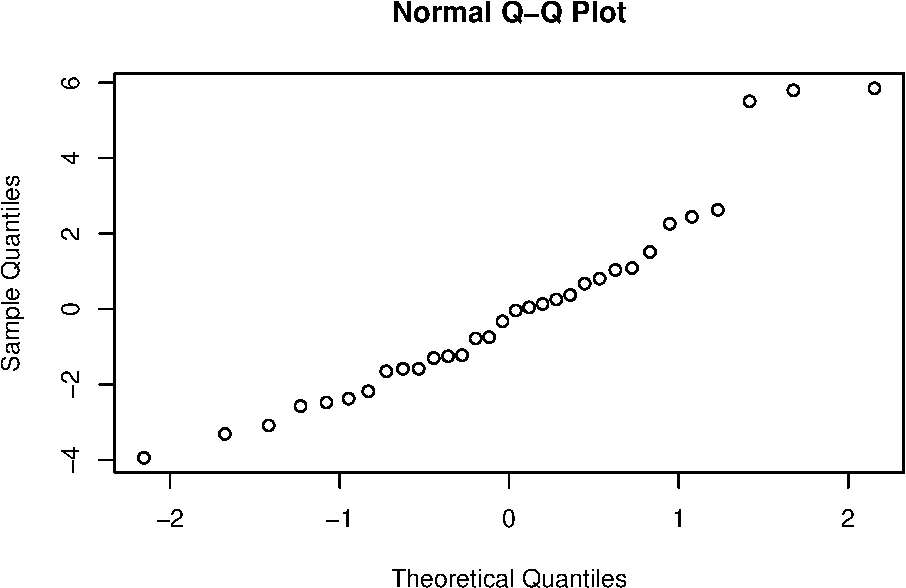
\includegraphics{hw3_files/figure-latex/unnamed-chunk-8-1.pdf} The
QQ-plot of the residuals is not quite a 45 degree line, suggesting that
the assumption of normality on the error term may not be reasonable
under some circumstances.

Next, we show the historgram of the residuals

\begin{Shaded}
\begin{Highlighting}[]
\CommentTok{\# construct a histogram plot of the residuals}
\FunctionTok{hist}\NormalTok{(mpg\_hp\_wt.model}\SpecialCharTok{$}\NormalTok{residual)}
\end{Highlighting}
\end{Shaded}

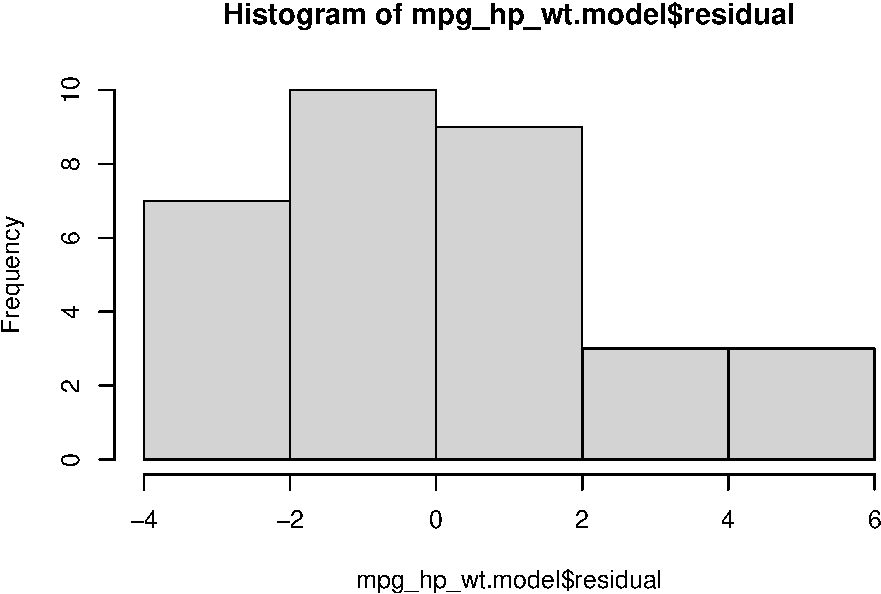
\includegraphics{hw3_files/figure-latex/unnamed-chunk-9-1.pdf} This is
not terribly symmetric, confirming our earlier suspicions.

\hypertarget{part-f-1}{%
\subsection{Part (F)}\label{part-f-1}}

\fbox{Obtain $\operatorname{SSR}(x_1)$, $\operatorname{SSR}(x_2|x_1)$, and verify $\operatorname{SSR}(x_1, x_2) = \operatorname{SSR}(x_1) + \operatorname{SSR}(x_2|x_1)$.}

The following R code generates the sum of squared regressions for the
models.

\begin{Shaded}
\begin{Highlighting}[]
\DocumentationTok{\#\#\#\# Testing on group of coefficients}
\NormalTok{result.full}\OtherTok{=}\FunctionTok{lm}\NormalTok{(mpg}\SpecialCharTok{\textasciitilde{}}\NormalTok{hp}\SpecialCharTok{+}\NormalTok{wt, }\AttributeTok{data=}\NormalTok{mtcars)}
\NormalTok{result.red\_x1}\OtherTok{=}\FunctionTok{lm}\NormalTok{(mpg}\SpecialCharTok{\textasciitilde{}}\NormalTok{hp, }\AttributeTok{data=}\NormalTok{mtcars)}
\NormalTok{result.red\_x2}\OtherTok{=}\FunctionTok{lm}\NormalTok{(mpg}\SpecialCharTok{\textasciitilde{}}\NormalTok{wt, }\AttributeTok{data=}\NormalTok{mtcars)}
\FunctionTok{summary}\NormalTok{(result.full)    }\CommentTok{\#get details from the regression output}
\end{Highlighting}
\end{Shaded}

\begin{verbatim}
## 
## Call:
## lm(formula = mpg ~ hp + wt, data = mtcars)
## 
## Residuals:
##    Min     1Q Median     3Q    Max 
## -3.941 -1.600 -0.182  1.050  5.854 
## 
## Coefficients:
##             Estimate Std. Error t value Pr(>|t|)    
## (Intercept) 37.22727    1.59879  23.285  < 2e-16 ***
## hp          -0.03177    0.00903  -3.519  0.00145 ** 
## wt          -3.87783    0.63273  -6.129 1.12e-06 ***
## ---
## Signif. codes:  0 '***' 0.001 '**' 0.01 '*' 0.05 '.' 0.1 ' ' 1
## 
## Residual standard error: 2.593 on 29 degrees of freedom
## Multiple R-squared:  0.8268, Adjusted R-squared:  0.8148 
## F-statistic: 69.21 on 2 and 29 DF,  p-value: 9.109e-12
\end{verbatim}

\begin{Shaded}
\begin{Highlighting}[]
\FunctionTok{anova}\NormalTok{(result.full)      }\CommentTok{\#ANOVA table for the full model}
\end{Highlighting}
\end{Shaded}

\begin{verbatim}
## Analysis of Variance Table
## 
## Response: mpg
##           Df Sum Sq Mean Sq F value    Pr(>F)    
## hp         1 678.37  678.37 100.862 5.987e-11 ***
## wt         1 252.63  252.63  37.561 1.120e-06 ***
## Residuals 29 195.05    6.73                      
## ---
## Signif. codes:  0 '***' 0.001 '**' 0.01 '*' 0.05 '.' 0.1 ' ' 1
\end{verbatim}

\begin{Shaded}
\begin{Highlighting}[]
\FunctionTok{anova}\NormalTok{(result.red\_x1)        }\CommentTok{\#ANOVA table for the reduced model}
\end{Highlighting}
\end{Shaded}

\begin{verbatim}
## Analysis of Variance Table
## 
## Response: mpg
##           Df Sum Sq Mean Sq F value    Pr(>F)    
## hp         1 678.37  678.37   45.46 1.788e-07 ***
## Residuals 30 447.67   14.92                      
## ---
## Signif. codes:  0 '***' 0.001 '**' 0.01 '*' 0.05 '.' 0.1 ' ' 1
\end{verbatim}

\begin{Shaded}
\begin{Highlighting}[]
\FunctionTok{anova}\NormalTok{(result.red\_x2)        }\CommentTok{\#ANOVA table for the reduced model}
\end{Highlighting}
\end{Shaded}

\begin{verbatim}
## Analysis of Variance Table
## 
## Response: mpg
##           Df Sum Sq Mean Sq F value    Pr(>F)    
## wt         1 847.73  847.73  91.375 1.294e-10 ***
## Residuals 30 278.32    9.28                      
## ---
## Signif. codes:  0 '***' 0.001 '**' 0.01 '*' 0.05 '.' 0.1 ' ' 1
\end{verbatim}

\begin{Shaded}
\begin{Highlighting}[]
\FunctionTok{anova}\NormalTok{(result.red\_x1,result.full,}\AttributeTok{test =} \StringTok{"F"}\NormalTok{) }\CommentTok{\#F{-}test for the effect of act and year togother}
\end{Highlighting}
\end{Shaded}

\begin{verbatim}
## Analysis of Variance Table
## 
## Model 1: mpg ~ hp
## Model 2: mpg ~ hp + wt
##   Res.Df    RSS Df Sum of Sq      F   Pr(>F)    
## 1     30 447.67                                 
## 2     29 195.05  1    252.63 37.561 1.12e-06 ***
## ---
## Signif. codes:  0 '***' 0.001 '**' 0.01 '*' 0.05 '.' 0.1 ' ' 1
\end{verbatim}

The sum of squares for the regression for the full model is
\(\operatorname{SSR}(x_1,x_2) = 930.996\). The sum of squares for the
regression when we remove \(x_1\) is
\(\operatorname{SSR}(x_2) = 847.7252\). The sum of squares for the
regression when we remove \(x_2\) is
\(\operatorname{SSR}(x_1) = 678.3729\). The extra sum of squares when we
add \(x_2\) given \(x_1\) is already in the model is
\(\operatorname{SSR}(x_2|x_1) = \operatorname{SSR}(x_1,x_2) - \operatorname{SSR}(x_1) = 930.996 - 678.3729 = 252.6266\).
Thus, plugging them in, \(930.996 = 678.3729+252.6266\).

\hypertarget{part-g}{%
\subsection{Part (G)}\label{part-g}}

\fbox{Obtain and interpret an $95\%$ interval estimate of $\operatorname{E}(Y_h)$ when $x_{h 1} = 100$ and $x_{h 2} = 4$.}

Look in the next section, Alternative approach to Problem 3, where I
compute the intervals. There's a lot of other stuff there, also, but the
intervals are near the end of the R code block.

I get the result \([16.66102, 20.41629]\).

\hypertarget{alternative-approach-to-problem-3}{%
\section{Alternative approach to Problem
3}\label{alternative-approach-to-problem-3}}

We use the matrix approach. Here is the R code.

\begin{Shaded}
\begin{Highlighting}[]
\DocumentationTok{\#\#\#\# Regression analysis using matrix methods \#\#\#\#}
\NormalTok{p3.Y }\OtherTok{\textless{}{-}}\NormalTok{ mtcars[}\FunctionTok{c}\NormalTok{(}\StringTok{"mpg"}\NormalTok{)]}
\FunctionTok{rownames}\NormalTok{(p3.Y) }\OtherTok{\textless{}{-}} \ConstantTok{NULL}
\FunctionTok{colnames}\NormalTok{(p3.Y) }\OtherTok{\textless{}{-}} \ConstantTok{NULL}
\NormalTok{p3.Y }\OtherTok{\textless{}{-}} \FunctionTok{data.matrix}\NormalTok{(p3.Y)}
\NormalTok{p3.n }\OtherTok{\textless{}{-}} \FunctionTok{nrow}\NormalTok{(p3.Y)}
\NormalTok{p3.X }\OtherTok{\textless{}{-}}\NormalTok{ mtcars[}\FunctionTok{c}\NormalTok{(}\StringTok{"hp"}\NormalTok{,}\StringTok{"wt"}\NormalTok{)]}
\FunctionTok{rownames}\NormalTok{(p3.X) }\OtherTok{\textless{}{-}} \ConstantTok{NULL}
\FunctionTok{colnames}\NormalTok{(p3.X) }\OtherTok{\textless{}{-}} \ConstantTok{NULL}
\NormalTok{p3.X }\OtherTok{\textless{}{-}} \FunctionTok{cbind}\NormalTok{(}\FunctionTok{rep}\NormalTok{(}\DecValTok{1}\NormalTok{,p3.n),}\FunctionTok{data.matrix}\NormalTok{(p3.X))}

\NormalTok{p3.XtX}\OtherTok{=}\FunctionTok{t}\NormalTok{(p3.X)}\SpecialCharTok{\%*\%}\NormalTok{p3.X       }\CommentTok{\#get X\textquotesingle{}X}
\NormalTok{p3.C}\OtherTok{=}\FunctionTok{solve}\NormalTok{(p3.XtX)}

\NormalTok{p3.coeffs}\OtherTok{=}\NormalTok{p3.C}\SpecialCharTok{\%*\%}\FunctionTok{t}\NormalTok{(p3.X)}\SpecialCharTok{\%*\%}\NormalTok{p3.Y }\CommentTok{\#Least Squares result}

\FunctionTok{print}\NormalTok{(p3.coeffs)}
\end{Highlighting}
\end{Shaded}

\begin{verbatim}
##             [,1]
## [1,] 37.22727012
## [2,] -0.03177295
## [3,] -3.87783074
\end{verbatim}

\begin{Shaded}
\begin{Highlighting}[]
\CommentTok{\# number of parameters p}
\NormalTok{p3.p }\OtherTok{\textless{}{-}} \DecValTok{3}

\CommentTok{\# degrees of freedom for SSR,SSE,and SST respectively}
\NormalTok{p3.df.r }\OtherTok{\textless{}{-}}\NormalTok{ p3.p}\DecValTok{{-}1}
\NormalTok{p3.df.e }\OtherTok{\textless{}{-}}\NormalTok{ p3.n}\SpecialCharTok{{-}}\NormalTok{p3.p}
\NormalTok{p3.df.t }\OtherTok{\textless{}{-}}\NormalTok{ p3.n}\DecValTok{{-}1}

\CommentTok{\# SSE = y\textquotesingle{}y {-} B\textquotesingle{}x\textquotesingle{}y}
\NormalTok{p3.ss.e}\OtherTok{=}\FunctionTok{t}\NormalTok{(p3.Y)}\SpecialCharTok{\%*\%}\NormalTok{p3.Y}\SpecialCharTok{{-}}\FunctionTok{t}\NormalTok{(p3.coeffs)}\SpecialCharTok{\%*\%}\FunctionTok{t}\NormalTok{(p3.X)}\SpecialCharTok{\%*\%}\NormalTok{p3.Y       }\CommentTok{\# calculate SSE}
\NormalTok{p3.ms.e}\OtherTok{=}\NormalTok{p3.ss.e}\SpecialCharTok{/}\NormalTok{p3.df.e }\CommentTok{\# calculate MSE}

\CommentTok{\# SSR = B\textquotesingle{}X\textquotesingle{}y {-} n avg(y)\^{}2}
\NormalTok{p3.ss.r}\OtherTok{=}\NormalTok{(}\FunctionTok{t}\NormalTok{(p3.coeffs)}\SpecialCharTok{\%*\%}\FunctionTok{t}\NormalTok{(p3.X)}\SpecialCharTok{\%*\%}\NormalTok{p3.Y}\SpecialCharTok{{-}}\NormalTok{p3.n}\SpecialCharTok{*}\FunctionTok{mean}\NormalTok{(p3.Y)}\SpecialCharTok{\^{}}\DecValTok{2}\NormalTok{)     }\CommentTok{\# calculate SSR}
\NormalTok{p3.ms.r}\OtherTok{=}\NormalTok{p3.ss.r}\SpecialCharTok{/}\NormalTok{p3.df.r                                 }\CommentTok{\# calculate MSR}

\CommentTok{\# SST = sum(y[i] {-} avg(y))}
\CommentTok{\#     = y\textquotesingle{}y {-} n*avg(y)}
\NormalTok{p3.ss.t}\OtherTok{=}\FunctionTok{t}\NormalTok{(p3.Y)}\SpecialCharTok{\%*\%}\NormalTok{p3.Y}\SpecialCharTok{{-}}\NormalTok{p3.n}\SpecialCharTok{*}\FunctionTok{mean}\NormalTok{(p3.Y)}\SpecialCharTok{\^{}}\DecValTok{2}                    \CommentTok{\# calculate SSTO}
\NormalTok{p3.ms.t}\OtherTok{=}\NormalTok{p3.ss.t}\SpecialCharTok{/}\NormalTok{p3.df.t}

\CommentTok{\# estimate of sigma\^{}2 is mean squared error (MSE)}
\NormalTok{p3.sigma2\_hat }\OtherTok{=}\NormalTok{ p3.ms.e}
\FunctionTok{print}\NormalTok{(p3.sigma2\_hat)}
\end{Highlighting}
\end{Shaded}

\begin{verbatim}
##          [,1]
## [1,] 6.725785
\end{verbatim}

\begin{Shaded}
\begin{Highlighting}[]
\CommentTok{\# covariance matrix for coefficient estimators}
\NormalTok{p3.cov}\OtherTok{=}\NormalTok{p3.sigma2\_hat[}\DecValTok{1}\NormalTok{]}\SpecialCharTok{*}\NormalTok{p3.C}
\FunctionTok{print}\NormalTok{(p3.C)}
\end{Highlighting}
\end{Shaded}

\begin{verbatim}
##               [,1]          [,2]          [,3]
## [1,]  3.800481e-01  2.207476e-05 -0.1094214557
## [2,]  2.207476e-05  1.212285e-05 -0.0005595912
## [3,] -1.094215e-01 -5.595912e-04  0.0595249024
\end{verbatim}

\begin{Shaded}
\begin{Highlighting}[]
\NormalTok{p3.r.sq}\OtherTok{=}\NormalTok{(}\FunctionTok{t}\NormalTok{(p3.coeffs)}\SpecialCharTok{\%*\%}\FunctionTok{t}\NormalTok{(p3.X)}\SpecialCharTok{\%*\%}\NormalTok{p3.Y}\SpecialCharTok{{-}}\NormalTok{p3.n}\SpecialCharTok{*}\FunctionTok{mean}\NormalTok{(p3.Y)}\SpecialCharTok{\^{}}\DecValTok{2}\NormalTok{)}\SpecialCharTok{/}\NormalTok{p3.ss.t  }\CommentTok{\# calculate R{-}square}
\FunctionTok{print}\NormalTok{(p3.r.sq)}
\end{Highlighting}
\end{Shaded}

\begin{verbatim}
##           [,1]
## [1,] 0.8267855
\end{verbatim}

\begin{Shaded}
\begin{Highlighting}[]
\NormalTok{p3.F.ratio}\OtherTok{=}\NormalTok{p3.ms.r}\SpecialCharTok{/}\NormalTok{p3.ms.e      }\CommentTok{\#F test for overall model significance}
\NormalTok{p3.pval}\OtherTok{=}\DecValTok{1}\SpecialCharTok{{-}}\FunctionTok{pf}\NormalTok{(p3.F.ratio,}\DecValTok{2}\NormalTok{,p3.n}\DecValTok{{-}3}\NormalTok{)   }\CommentTok{\#p{-}value from the F test}

\NormalTok{p3.anova }\OtherTok{\textless{}{-}} \FunctionTok{data.frame}\NormalTok{(}
   \AttributeTok{type =} \FunctionTok{c}\NormalTok{(}\StringTok{"regression"}\NormalTok{,}\StringTok{"residual"}\NormalTok{,}\StringTok{"total"}\NormalTok{), }
   \AttributeTok{ss =} \FunctionTok{c}\NormalTok{(p3.ss.r,p3.ss.e,p3.ss.t),}
   \AttributeTok{dof=}\FunctionTok{c}\NormalTok{(p3.df.r,p3.df.e,p3.df.t),}
   \AttributeTok{ms =} \FunctionTok{c}\NormalTok{(p3.ms.r,p3.ms.e,p3.ms.t)}
\NormalTok{)}
\NormalTok{knitr}\SpecialCharTok{::}\FunctionTok{kable}\NormalTok{(p3.anova, }\AttributeTok{digits=}\DecValTok{2}\NormalTok{, }\AttributeTok{caption =} \StringTok{"ANOVA table."}\NormalTok{)}
\end{Highlighting}
\end{Shaded}

\begin{longtable}[]{@{}lrrr@{}}
\caption{ANOVA table.}\tabularnewline
\toprule\noalign{}
type & ss & dof & ms \\
\midrule\noalign{}
\endfirsthead
\toprule\noalign{}
type & ss & dof & ms \\
\midrule\noalign{}
\endhead
\bottomrule\noalign{}
\endlastfoot
regression & 931.00 & 2 & 465.50 \\
residual & 195.05 & 29 & 6.73 \\
total & 1126.05 & 31 & 36.32 \\
\end{longtable}

\begin{Shaded}
\begin{Highlighting}[]
\NormalTok{p3.B0.est }\OtherTok{=}\NormalTok{ p3.coeffs[}\DecValTok{1}\NormalTok{]}
\NormalTok{p3.B0.se }\OtherTok{=} \FunctionTok{sqrt}\NormalTok{(p3.ms.e}\SpecialCharTok{*}\NormalTok{p3.C[}\DecValTok{1}\NormalTok{,}\DecValTok{1}\NormalTok{])}

\NormalTok{p3.B1.est }\OtherTok{=}\NormalTok{ p3.coeffs[}\DecValTok{2}\NormalTok{]}
\NormalTok{p3.B1.se }\OtherTok{=} \FunctionTok{sqrt}\NormalTok{(p3.ms.e}\SpecialCharTok{*}\NormalTok{p3.C[}\DecValTok{2}\NormalTok{,}\DecValTok{2}\NormalTok{])}

\NormalTok{p3.B2.est }\OtherTok{=}\NormalTok{ p3.coeffs[}\DecValTok{3}\NormalTok{]}
\NormalTok{p3.B2.se }\OtherTok{=} \FunctionTok{sqrt}\NormalTok{(p3.ms.e}\SpecialCharTok{*}\NormalTok{p3.C[}\DecValTok{3}\NormalTok{,}\DecValTok{3}\NormalTok{])}

\NormalTok{p3.B0.t0 }\OtherTok{\textless{}{-}}\NormalTok{ p3.B0.est }\SpecialCharTok{/}\NormalTok{ p3.B0.se}
\NormalTok{p3.B1.t0 }\OtherTok{\textless{}{-}}\NormalTok{ p3.B1.est }\SpecialCharTok{/}\NormalTok{ p3.B1.se}
\NormalTok{p3.B2.t0 }\OtherTok{\textless{}{-}}\NormalTok{ p3.B2.est }\SpecialCharTok{/}\NormalTok{ p3.B2.se}


\FunctionTok{cat}\NormalTok{(}\StringTok{"overall F0 ="}\NormalTok{,p3.F.ratio,}\StringTok{"pval ="}\NormalTok{,p3.pval)}
\end{Highlighting}
\end{Shaded}

\begin{verbatim}
## overall F0 = 69.21121 pval = 9.109047e-12
\end{verbatim}

\begin{Shaded}
\begin{Highlighting}[]
\FunctionTok{cat}\NormalTok{(}\StringTok{"B0 ="}\NormalTok{,p3.B0.est,}\StringTok{"se(B0) ="}\NormalTok{,p3.B0.se,}\StringTok{"t0 ="}\NormalTok{,p3.B0.t0)}
\end{Highlighting}
\end{Shaded}

\begin{verbatim}
## B0 = 37.22727 se(B0) = 1.598788 t0 = 23.28469
\end{verbatim}

\begin{Shaded}
\begin{Highlighting}[]
\FunctionTok{cat}\NormalTok{(}\StringTok{"B1 ="}\NormalTok{,p3.B1.est,}\StringTok{"se(B1) ="}\NormalTok{,p3.B1.se,}\StringTok{"t0 ="}\NormalTok{,p3.B1.t0)}
\end{Highlighting}
\end{Shaded}

\begin{verbatim}
## B1 = -0.03177295 se(B1) = 0.00902971 t0 = -3.518712
\end{verbatim}

\begin{Shaded}
\begin{Highlighting}[]
\FunctionTok{cat}\NormalTok{(}\StringTok{"B2 ="}\NormalTok{,p3.B2.est,}\StringTok{"se(B2) ="}\NormalTok{,p3.B2.se,}\StringTok{"t0 ="}\NormalTok{,p3.B2.t0)}
\end{Highlighting}
\end{Shaded}

\begin{verbatim}
## B2 = -3.877831 se(B2) = 0.6327335 t0 = -6.128695
\end{verbatim}

\begin{Shaded}
\begin{Highlighting}[]
\DocumentationTok{\#\#\#\#\# code for confidence intervals}
\NormalTok{x0 }\OtherTok{\textless{}{-}} \FunctionTok{c}\NormalTok{(}\DecValTok{1}\NormalTok{,}\DecValTok{100}\NormalTok{,}\DecValTok{4}\NormalTok{)}
\NormalTok{yhat}\OtherTok{=}\FunctionTok{t}\NormalTok{(p3.coeffs)}\SpecialCharTok{\%*\%}\NormalTok{x0}
\FunctionTok{print}\NormalTok{(yhat)}
\end{Highlighting}
\end{Shaded}

\begin{verbatim}
##          [,1]
## [1,] 18.53865
\end{verbatim}

\begin{Shaded}
\begin{Highlighting}[]
\NormalTok{se.yhat}\OtherTok{=}\FunctionTok{sqrt}\NormalTok{(p3.ms.e}\SpecialCharTok{*}\FunctionTok{t}\NormalTok{(x0)}\SpecialCharTok{\%*\%}\NormalTok{p3.C}\SpecialCharTok{\%*\%}\NormalTok{x0)     }\CommentTok{\#std.error for the mean response}
\NormalTok{CI.l}\OtherTok{=}\NormalTok{yhat}\SpecialCharTok{{-}}\FunctionTok{qt}\NormalTok{(}\FloatTok{0.975}\NormalTok{,n}\DecValTok{{-}3}\NormalTok{)}\SpecialCharTok{*}\NormalTok{se.yhat}
\NormalTok{CI.u}\OtherTok{=}\NormalTok{yhat}\SpecialCharTok{+}\FunctionTok{qt}\NormalTok{(}\FloatTok{0.975}\NormalTok{,n}\DecValTok{{-}3}\NormalTok{)}\SpecialCharTok{*}\NormalTok{se.yhat     }\CommentTok{\#the lower/upper limit for a 95\% CI}
\FunctionTok{print}\NormalTok{(CI.l)}
\end{Highlighting}
\end{Shaded}

\begin{verbatim}
##          [,1]
## [1,] 16.66102
\end{verbatim}

\begin{Shaded}
\begin{Highlighting}[]
\FunctionTok{print}\NormalTok{(CI.u)}
\end{Highlighting}
\end{Shaded}

\begin{verbatim}
##          [,1]
## [1,] 20.41629
\end{verbatim}

We collect the results and summarize the results in the following table:

\begin{longtable}[]{@{}lllll@{}}
\caption{Coefficient statistics}\tabularnewline
\toprule\noalign{}
& \(\hat\beta_j\) & \(\operatorname{SE}(\hat\beta_j)\) & \(t_0\) &
\(F_0\) \\
\midrule\noalign{}
\endfirsthead
\toprule\noalign{}
& \(\hat\beta_j\) & \(\operatorname{SE}(\hat\beta_j)\) & \(t_0\) &
\(F_0\) \\
\midrule\noalign{}
\endhead
\bottomrule\noalign{}
\endlastfoot
\(\beta_0\) & 37.22727 & 1.598788 & 23.28469 & 69.21121 \\
\(\beta_1\) & -0.03177295 & 0.00902971 & -3.518712 & \\
\(\beta_2\) & -3.877831 & 0.6327335 & -6.128695 & \\
\end{longtable}

\end{document}
